% \newpage
\section{More results on text reasoning task}
\label{app:Text-Cases}
\begin{figure}[htbp]
\centering
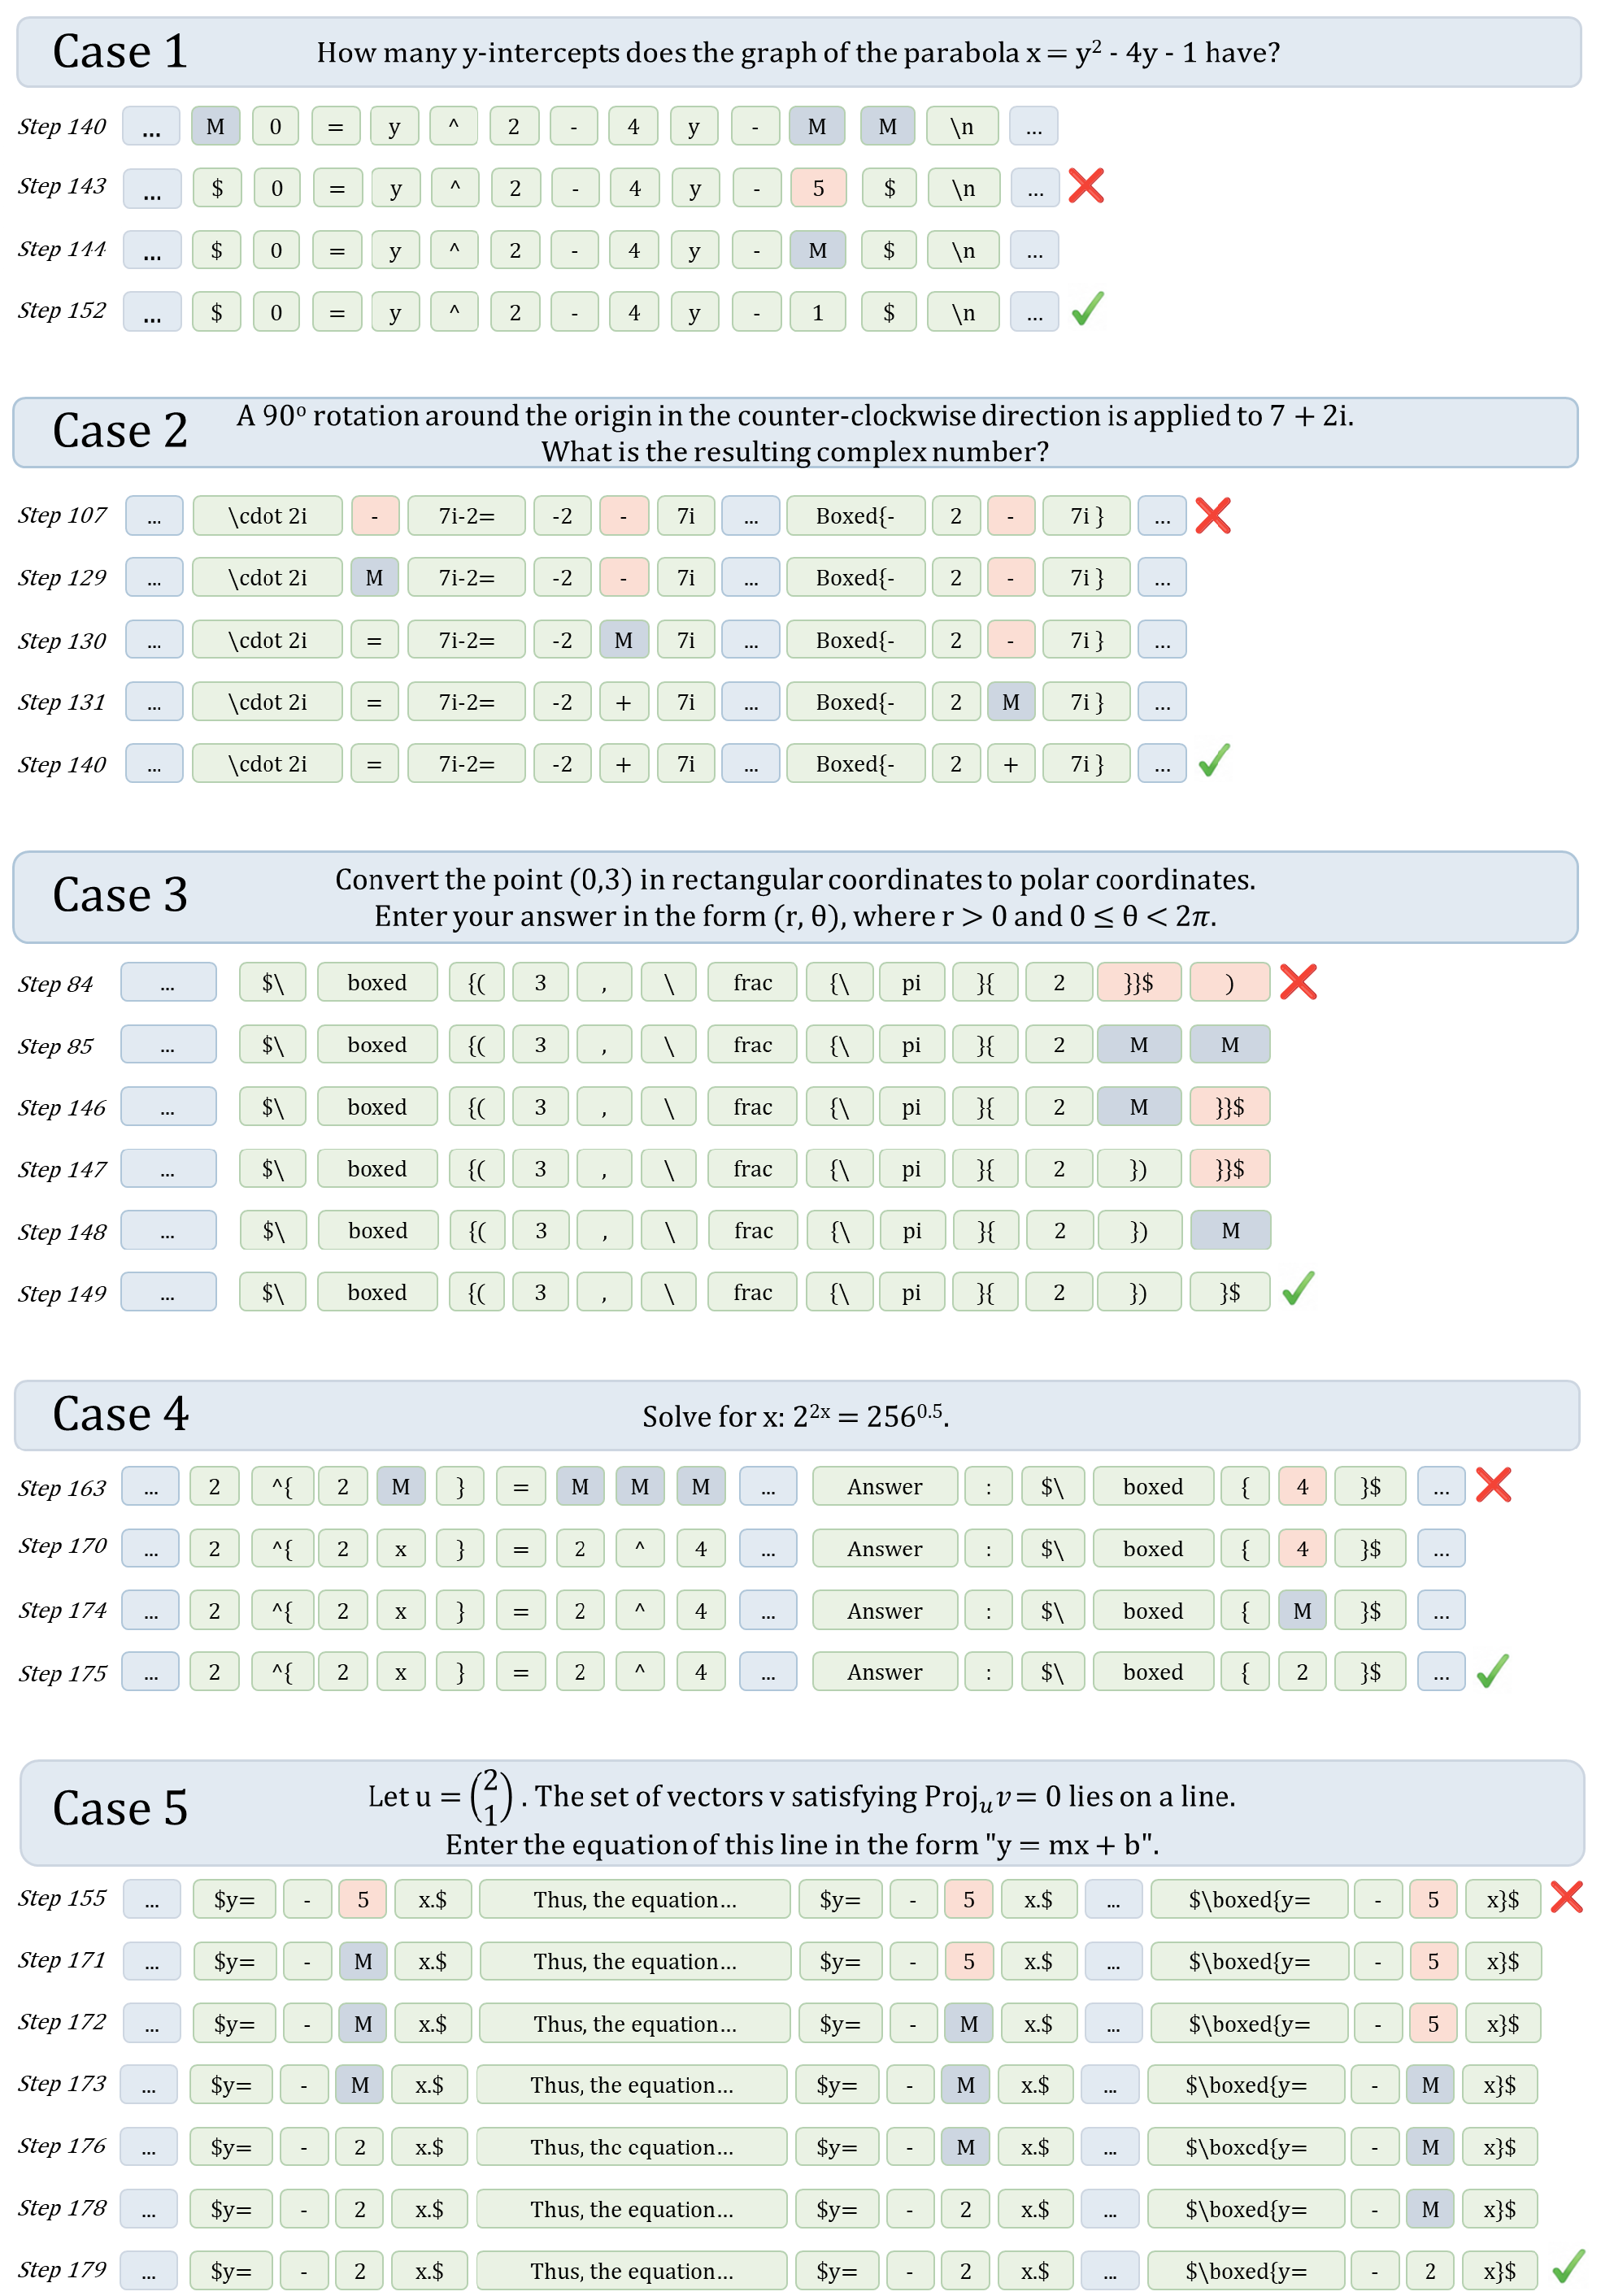
\includegraphics[width=0.96\linewidth]{figures/text_case_appendix_img.pdf}
\caption{
\textbf{Additional qualitative results on text generation.}
}
\label{app_text:Text_result_gallery}
\end{figure}

Fig.~\ref{app_text:Text_result_gallery} shows additional text revisions from our experiments. Cases 1 and 4: the model re-masks a token that is logically inconsistent with its surrounding context and re-predicts it. Cases 2 and 5: a single corrected token cascades downstream. After the earlier position is revised, the model also re-masks dependent positions further to the right and re-predicts them to be consistent with the corrected context. Case 3: format-level correction, where re-masking targets tokens whose surface form violates the answer template.